\documentclass[12pt]{article}
\usepackage{amsmath}
\title{EECS 440: HW 1}
\author{Justin Gray}

\setlength{\parindent}{0pt}
\setlength{\parskip}{1ex plus 0.5ex minus 0.2ex}

\usepackage{graphicx}
\usepackage{float}

\begin{document}

\maketitle

1)Suppose f and g are two convex functions defined on $R^n$. Show that the following functions are also convex: (i) $h(x)=f(x)+g(x)$, 
(ii) $h(x)=max(f(x),g(x))$.

Jensen's Inequality states that $f(\lambda x_1  +(1-\lambda)x_2) \leq \lambda f(x_1)+(1-\lambda)f(x_2)$  

\begin{align}  
f(\lambda x_1  +(1-\lambda)x_2 ) &\leq \lambda f(x_1)+(1-\lambda)f(x_2)\\
g(\lambda x_1  +(1-\lambda)x_2 ) &\leq \lambda g(x_1)+(1-\lambda)g(x_2)
\end{align} 

i)$h(x)=f(x)+g(x)$


Applying Jensen's inequality to h(x) yeilds: 
\begin{equation}
h(\lambda x_1  + (1 − \lambda) x_2 ) \leq \lambda h(x_1)+(1-\lambda)h(x_2)
\end{equation}
\begin{align}
    \lambda h(x_1) &= \lambda f(x_1) + \lambda g(x_1) \\
    (1-\lambda)h(x_2) &= (1-\lambda)f(x_2) + (1-\lambda)g(x_2) \\
    h(\lambda x_1  +(1−\lambda)x_2) &= f(\lambda x_1  +(1-\lambda)x_2) + g(\lambda x_1  +(1-\lambda)x_2)    
\end{align}

Combining eqns. 3,4,5,6 yeilds: 
\begin{align}
f(\lambda x_1  +(1-\lambda)x_2 ) + g(\lambda x_1  +(1-\lambda)x_2 ) \leq \\
\lambda f(x_1)+(1-\lambda)f(x_2) + \lambda g(x_1)+(1-\lambda)g(x_2) \notag
\end{align}
Since we know eqn. 1 \& 2 hold, you it is clear that the combined inequallity will also be true. Hence, h(x) is convex

Alternatively, if $f(x)$ and $g(x)$ are both convex, then $f\prime\prime(x) \geq 0$  and $g\prime\prime(x) \geq 0$. So for $h(x) = f(x) + g(x)$
then $h\prime\prime(x) = f\prime\prime(x) + g\prime\prime(x)$. Since both $f\prime\prime(x)$ and $g\prime\prime(x)$ are known to be greater than 
or equal to 0, $h\prime\prime(x)$ must also be. Hence h(x) is also convex. 


ii) $h(x)=max(f(x),g(x))$

Applying Jensen's inequality to h(x) yeilds: 
\begin{equation}
h(\lambda x_1  + (1 − \lambda) x_2 ) \leq \lambda h(x_1)+(1-\lambda)h(x_2)
\end{equation}
\begin{align}
    \lambda h(x_1) &= \lambda max\left(f(x_1),g(x_1)\right) \\
    (1-\lambda) h(x_2) &= (1-\lambda) \max \left(f(x_2),g(x_2)\right) \\
    h(\lambda x_1  +(1−\lambda)x_2) &= \max \left( f(\lambda x_1  +(1-\lambda)x_2),g(\lambda x_1  +(1-\lambda)x_2)\right)    
\end{align}

combining eqns. 8,9,10,11 yeilds: 
\begin{align}
\max \left( f(\lambda x_1  +(1-\lambda)x_2),g(\lambda x_1  +(1-\lambda)x_2)\right) \leq \\
\lambda max\left(f(x_1),g(x_1)\right) + (1-\lambda) \max \left(f(x_2),g(x_2)\right) \notag
\end{align}

In eqn. 12, from the left hand side, either $f(\lambda x_1  +(1-\lambda)x_2)$ will be greater, or 
$g(\lambda x_1  +(1-\lambda)x_2)$ will be. Without loss of generality, assume that 
$g(\lambda x_1  +(1-\lambda)x_2)$ is greater. There are three possible outcomes: \\

A)From the right hand side of eqn 12, if you assume that $g(x_1) > f(x_1)$ and $g(x_2) > f(x_2)$ 
then eqn 12 reduces down to 
\begin{equation*}
g(\lambda x_1  +(1-\lambda)x_2 ) \leq \lambda g(x_1)+(1-\lambda)g(x_2)
\end{equation*}
which is equivilent to eqn. 2, and h(x) must be convex. \\

B)From the right hand side of eqn 12, if you assume that $g(x_1) < f(x_1)$ and $g(x_2) < f(x_2)$ 
then eqn 12 reduces down to
\begin{equation*}
g(\lambda x_1  +(1-\lambda)x_2 ) \leq \lambda f(x_1)+(1-\lambda)f(x_2)
\end{equation*}
However, since you know that $g(x_1) < f(x_1)$ and $g(x_2) < f(x_2)$, then: 
\begin{equation*}
\lambda f(x_1)+(1-\lambda)f(x_2) \geq \lambda g(x_1)+(1-\lambda)g(x_2)
\end{equation*}
so eqn 12 reduces to eqn 2, so h(x) must be convex. \\

B)From the right hand side of eqn 12, if you assume that $g(x_1) > f(x_1)$ but $g(x_2) < f(x_2)$ 
then eqn 12 reduces down to
\begin{equation*}
g(\lambda x_1  +(1-\lambda)x_2 ) \leq \lambda g(x_1)+(1-\lambda)f(x_2)
\end{equation*}
however, again since you know that $g(x_2) < f(x_2)$, then: 
\begin{equation*}
\lambda g(x_1)+(1-\lambda)g(x_2) \leq \lambda g(x_1)+(1-\lambda)f(x_2)
\end{equation*}
so again, h(x) must be convex. \\

Since h(x) is convex for all three outcomes (and obviously true for the alternate case when
$f(\lambda x_1  +(1-\lambda)x_2)$), then h(x) is always convex.

\pagebreak
\setcounter{equation}{0}
2) Show that the set $C=\{x|Ax \geq b\} , A\ in\ R^{m \times n}, x,b\ in\ R^n$, is a convex set. Note that this describes the constraint set of a linear program.

A set is convex if for any $x_1,x_2$ in $C$, $\lambda x_1 + (1-\lambda)x_2$ is also in $C$.
For the set $C=\{x|Ax \geq b\}$ to be convex, then: 
\begin{equation}
    A(\lambda x_1 + (1-\lambda)x_2) \geq b
\end{equation}
which is equivilent to 
\begin{equation}
    A \lambda x_1 + A(1-\lambda)x_2 \geq b
\end{equation}

We know that for any $x$ which belongs to $C$, $Ax \geq b$ will hold. Hence 
either $A \lambda x_1 \geq b$ (for $\lambda |\lambda \neq 0$) and 
$A(1-\lambda)x_2 \geq b$ (for $\lambda |\lambda \neq 1$). So the sum of these two quantities 
for any $\lambda$ must also be greater than $b$. Hence, eqn 1 is proven valid and 
the set $C$ is complex. 

\pagebreak
\setcounter{equation}{0}
3)Consider the primal LP: $\min c^T x \ s.t. \ Ax \geq b, x \geq 0$ and its 
dual: $\max b^Tu \ s.t. \ A^Tu \leq c, u \geq 0$. Prove that for any feasible (x,u) 
(i.e. x and u satisfying the constraints of the two LPs), $b^Tu \leq c^Tx$. 

For the primal, multiplying both sides of the constraint by $u^T$: 
\begin{equation}
    u^TAx \geq u^Tb
\end{equation}

For the dual, first take the transpose of both sides: 
\begin{equation}
    u^TA \leq c^T
\end{equation}
Next, multiply both sides by $x$
\begin{equation}
    u^TAx \leq c^Tx
\end{equation}

hence: 
\begin{align}
  c^Tx \geq u^TAx \geq u^Tb \\
  c^Tx \geq u^Tb \notag
\end{align}
note that:
\begin{equation}
  bu^T = u^Tb 
\end{equation}
so: 
\begin{equation}
c^Tx \geq bu^T
\end{equation}


\pagebreak
\setcounter{equation}{0}
a)
\begin{figure}[H]
 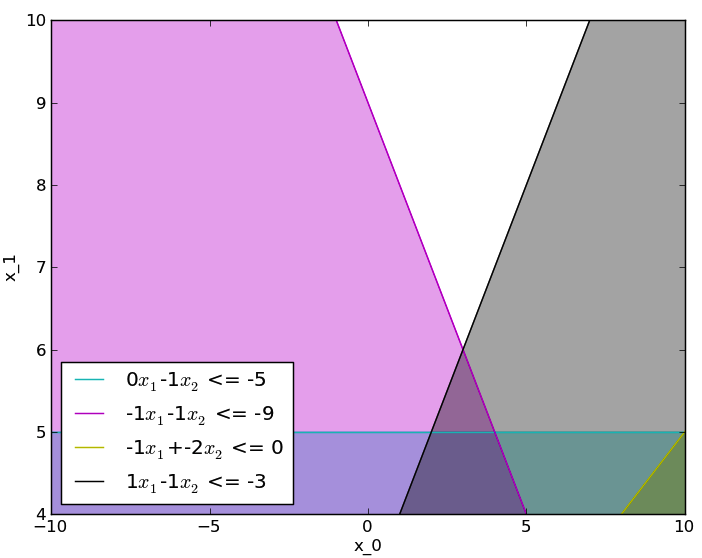
\includegraphics[width=\textwidth]{4_a}
\end{figure}
\pagebreak
b)
\begin{figure}[H]
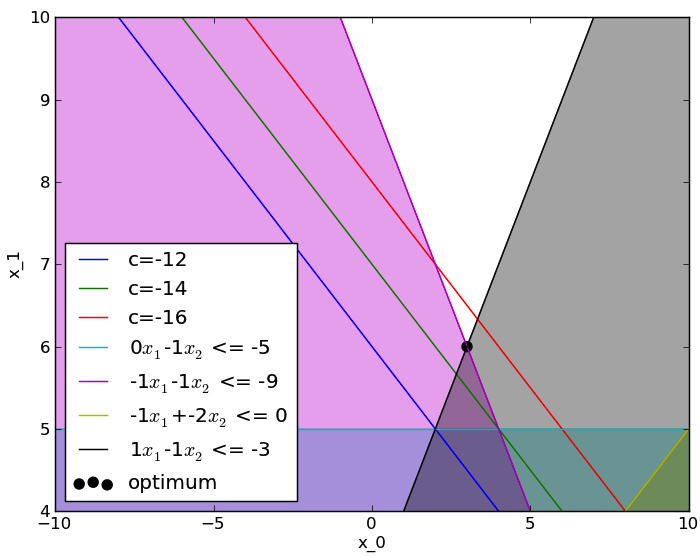
\includegraphics[width=\textwidth]{4_b}
\end{figure}
\pagebreak
c)
\begin{figure}[H]
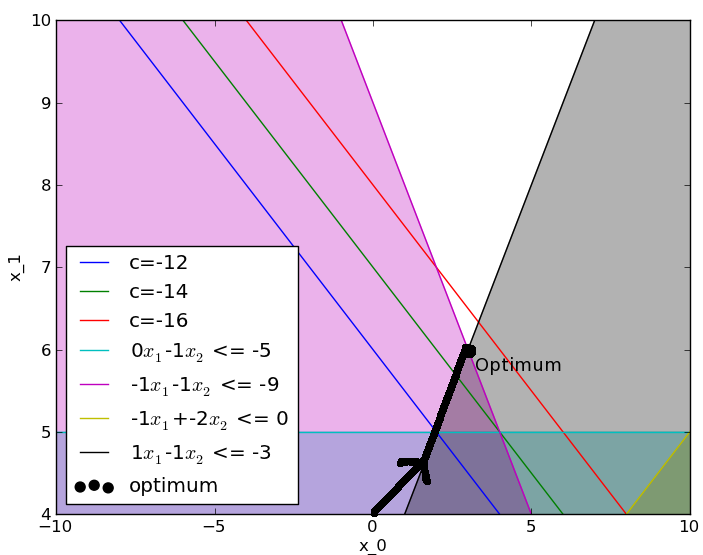
\includegraphics[width=\textwidth]{4_c}
\end{figure}

\pagebreak
\setcounter{equation}{0}
5) A function f is said to have a global minimum at x if for all y, 
$f(y) \geq f(x)$. It is said to have a local minimum at x if there 
exists a neighborhood H around x so that for all y in H, $f(y) \geq f(x)$. 
Show that, if f is convex, every local minimum is a global minimum. 

assume that you have a local minimum at $x^*$, so that for y in H, $f(y) \geq f(x)$. If you 
examine a point, p, at $\lambda y  + (1-\lambda)x^*$. If you make the value for $\lambda$
sufficently small, then p will be in H. So you know that

\begin{equation}
    f(x^*) \leq f(\lambda y  + (1-\lambda)x^*) 
\end{equation}

from the definition of convexity: 

\begin{equation}
    f(\lambda y  + (1-\lambda)x^*) \leq \lambda f(y) + (1-\lambda) f(x^*)
\end{equation}

combining eqn. 1 and 2, then rearanging terms 
\begin{align}
    f(x^*) &\leq f(\lambda y  + (1-\lambda)x^*) \leq \lambda f(y) + (1-\lambda) f(x^*) \\
    f(x^*) &\leq \lambda f(y) + (1-\lambda) f(x^*) \\ \notag
    f(x^*) &\leq \lambda f(y) + f(x^*) - \lambda f(x^*)\\ \notag
    f(x^*) &\leq f(y)\\ \notag
\end{align}
hence, for any local optimum when teh function is convex, it is a global optimum. 
\end{document}